\documentclass{article}
\usepackage[utf8]{inputenc}
\usepackage{graphicx}
\usepackage{subcaption}
\usepackage{hyperref}
\captionsetup[subfigure]{labelformat=empty}
\graphicspath{ {./images/} }

% Use geometry to control margin sizes
\usepackage[top=0.5in, bottom=0.5in, left=1in, right=1in]{geometry}

\usepackage{array}
\usepackage{color}
\usepackage{booktabs}

% Title, Author, and Date
\title{NTU AI 2024 HW1 Report}
\author{B10902037 Yu Xiang Luo}
\date{}

\begin{document}

\maketitle

\[
	\textcolor{red}{\textbf{\textit{Detail can be found in: }}}
	\href{https://github.com/YuXiangLo/NTUAI2024}{here}
\]

\section*{Task 1}

\begin{enumerate}
    \item Briefly describe how you implement the two models: \\
		\\
		In this assignment, I utilize the huggingface packages to conduct the experiments. Below is the main package I use:
        \begin{itemize}
            \item \textcolor{blue}{\texttt{transformer.AutoModel...}} $\rightarrow$ Load models.
            \item \textcolor{blue}{\texttt{datasets.load\_dataset}} $\rightarrow$ Load datasets.
            \item \textcolor{blue}{\texttt{torch.utils.data.DataLoader}} $\rightarrow$ Process data in batch to inference faster.
			\item \textcolor{blue}{\texttt{evaluate}} $\rightarrow$ Provide functions for Corpus BLEU, ROUGE, and METEOR.
        \end{itemize}
		I also converted the captions to lowercase and removed punctuation for better evaluations.\\

    \item Metrics Result:
        \begin{table}[ht]
        \centering
        \begin{tabular}{l cccc cccc}
        \toprule
         & \multicolumn{4}{c}{MSCOCO-Test} & \multicolumn{4}{c}{flickr30k}\\
        \cmidrule(lr){2-5} \cmidrule(lr){6-9}
         & BLEU & ROUGE-1 & ROUGE-2 & METEOR & BLEU & ROUGE-1 & ROUGE-2 & METEOR \\
        \midrule
        BLIP  & 0.3237 & 0.4023 & 0.1594 & 0.2776 & 0.2398 & 0.3206 & 0.1091 & 0.2033 \\
        Phi-4 & 0.2560 & 0.3971 & 0.1517 & 0.3325 & 0.2658 & 0.3636 & 0.1400 & 0.3043 \\
        \bottomrule
        \end{tabular}
        \end{table}

	\item Analysis:
	\begin{itemize}
		\item In the MSCOCO experiments, BLIP outperforms Phi-4 on BLEU metrics but is outperformed by Phi-4 on METEOR. This suggests that BLIP's output aligns more closely with the specific wording used by MSCOCO annotators, leading to higher BLEU scores. In contrast, Phi-4, as a larger model, likely generates captions with a more diverse vocabulary, improving its METEOR score by capturing broader semantic similarities.
		
		\item In the Flickr30k experiments, Phi-4 outperforms BLIP across all metrics, indicating that Phi-4 is more effective for this dataset.

		\item Comparing the two datasets, we observe that the overall metric scores are higher for MSCOCO, suggesting differences in dataset complexity, with MSCOCO potentially being easier for models to perform well on.\\ 
	\end{itemize}

	\item Case Study: \\
		\\ 
		In Figure 1-a, the BLIP model generated the caption: \textit{``a man in a white shirt,''} which fails to mention that there are actually five men in the image. In contrast, the Phi-4 model produced the caption: \textit{``Men in business attire are standing around a van,''} which captures more detail and provides a more accurate description. However, when comparing these outputs to the reference captions, BLIP surprisingly achieved higher ROUGE-2 and METEOR scores than Phi-4. This example highlights a key limitation of rule-based language metrics: they tend to prioritize surface-level similarity and rigid sentence structures over semantic richness. In contrast, evaluating caption quality using cosine similarity between text embeddings could offer a more robust and meaningful measure of semantic alignment.
	\newpage
	\begin{figure}[h!]
		\centering

		\begin{subfigure}[t]{0.3\textwidth} % Note [t] for top alignment
			\centering
			\fbox{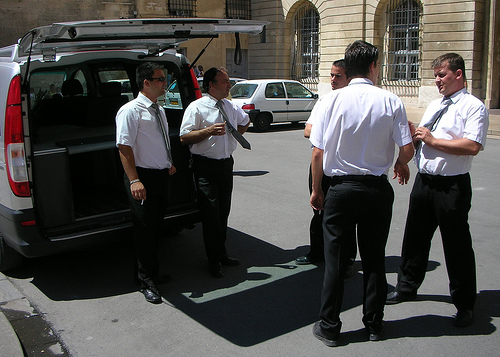
\includegraphics[height=3.5cm]{1010031975}}
			\caption{Figure 1-a: flickr30k image}
		\end{subfigure}
		\hfill
		\begin{subfigure}[t]{0.3\textwidth}
			\centering
			\fbox{
\includegraphics[height=3.5cm]{me_diff3}}
			\caption{Figure 1-b: Peanuts style by stable diffusion v3}
		\end{subfigure}
		\hfill
		\begin{subfigure}[t]{0.3\textwidth}
			\centering
			\fbox{
\includegraphics[height=3.5cm]{me_styled}}
			\caption{Figure 1-c: Peanuts style by stable diffusion v1.5}
		\end{subfigure}
	\end{figure}

\end{enumerate}

\section*{Task 2-1}
\begin{enumerate}
	\item Briefly describe how you implement task 2-1:
		\begin{itemize}
			\item Generated captions with Phi-4 beforehand and stored in a json file.
			\item Used \textcolor{blue}{\texttt{diffusers.StableDiffusion3Pipeline}}.
		\end{itemize}
	\item Visualization:
		\begin{enumerate}
			\item Figure 1-b shows an example output.
			\item Below are examples of success and failure. In the success samples, the images are indeed in the Peanuts style, and the hair color, hairstyle, clothes, and accessories are correctly generated. On the other hand, some failure samples show no Peanuts style at all.
				\begin{figure}[h!]
					\centering
					\begin{minipage}{0.8\textwidth}
						\centering

						% Row 1
						\begin{subfigure}[b]{0.18\textwidth}
							\centering
							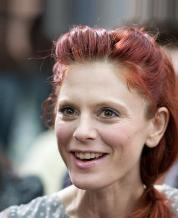
\includegraphics[height=1.9cm]{000002}
						\end{subfigure}
						\hfill
						\begin{subfigure}[b]{0.18\textwidth}
							\centering
							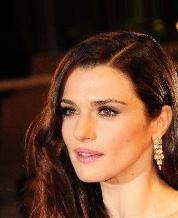
\includegraphics[height=1.9cm]{000073}
						\end{subfigure}
						\hfill
						\begin{subfigure}[b]{0.18\textwidth}
							\centering
							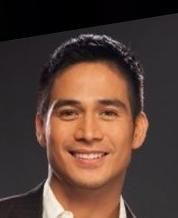
\includegraphics[height=1.9cm]{000012}
						\end{subfigure}
						\hfill
						\begin{subfigure}[b]{0.18\textwidth}
							\centering
							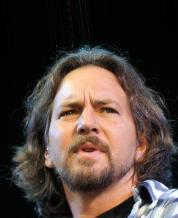
\includegraphics[height=1.9cm]{000020}
						\end{subfigure}
						\hfill
						\begin{subfigure}[b]{0.18\textwidth}
							\centering
							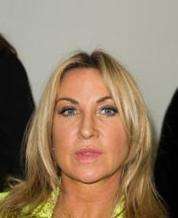
\includegraphics[height=1.9cm]{000022}
						\end{subfigure}

						\vspace{0.6cm} % Space between rows

						% Row 2
						\begin{subfigure}[b]{0.18\textwidth}
							\centering
							
\includegraphics[height=1.9cm]{000002_diff3}
						\end{subfigure}
						\hfill
						\begin{subfigure}[b]{0.18\textwidth}
							\centering
							
\includegraphics[height=1.9cm]{000073_diff3}
						\end{subfigure}
						\hfill
						\begin{subfigure}[b]{0.18\textwidth}
							\centering
							
\includegraphics[height=1.9cm]{000012_diff3}
						\end{subfigure}
						\hfill
						\begin{subfigure}[b]{0.18\textwidth}
							\centering
							
\includegraphics[height=1.9cm]{000020_diff3}
						\end{subfigure}
						\hfill
						\begin{subfigure}[b]{0.18\textwidth}
							\centering
							
\includegraphics[height=1.9cm]{000022_diff3}
						\end{subfigure}

						\caption{Task 2-1: Success samples}
						\vspace{0.6cm} % Space between rows

						% Row 1
						\begin{subfigure}[b]{0.18\textwidth}
							\centering
							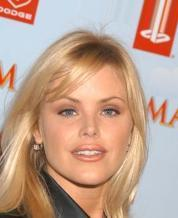
\includegraphics[height=1.9cm]{000029}
						\end{subfigure}
						\hfill
						\begin{subfigure}[b]{0.18\textwidth}
							\centering
							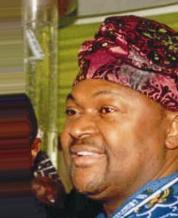
\includegraphics[height=1.9cm]{000060}
						\end{subfigure}
						\hfill
						\begin{subfigure}[b]{0.18\textwidth}
							\centering
							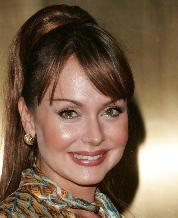
\includegraphics[height=1.9cm]{000009}
						\end{subfigure}
						\hfill
						\begin{subfigure}[b]{0.18\textwidth}
							\centering
							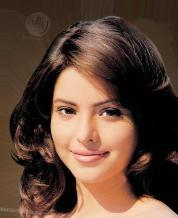
\includegraphics[height=1.9cm]{000077}
						\end{subfigure}
						\hfill
						\begin{subfigure}[b]{0.18\textwidth}
							\centering
							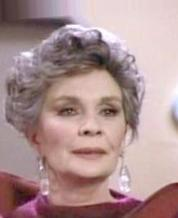
\includegraphics[height=1.9cm]{000084}
						\end{subfigure}

						\vspace{0.6cm} % Space between rows

						% Row 2
						\begin{subfigure}[b]{0.18\textwidth}
							\centering
							
\includegraphics[height=1.9cm]{000029_diff3}
						\end{subfigure}
						\hfill
						\begin{subfigure}[b]{0.18\textwidth}
							\centering
							
\includegraphics[height=1.9cm]{000060_diff3}
						\end{subfigure}
						\hfill
						\begin{subfigure}[b]{0.18\textwidth}
							\centering
							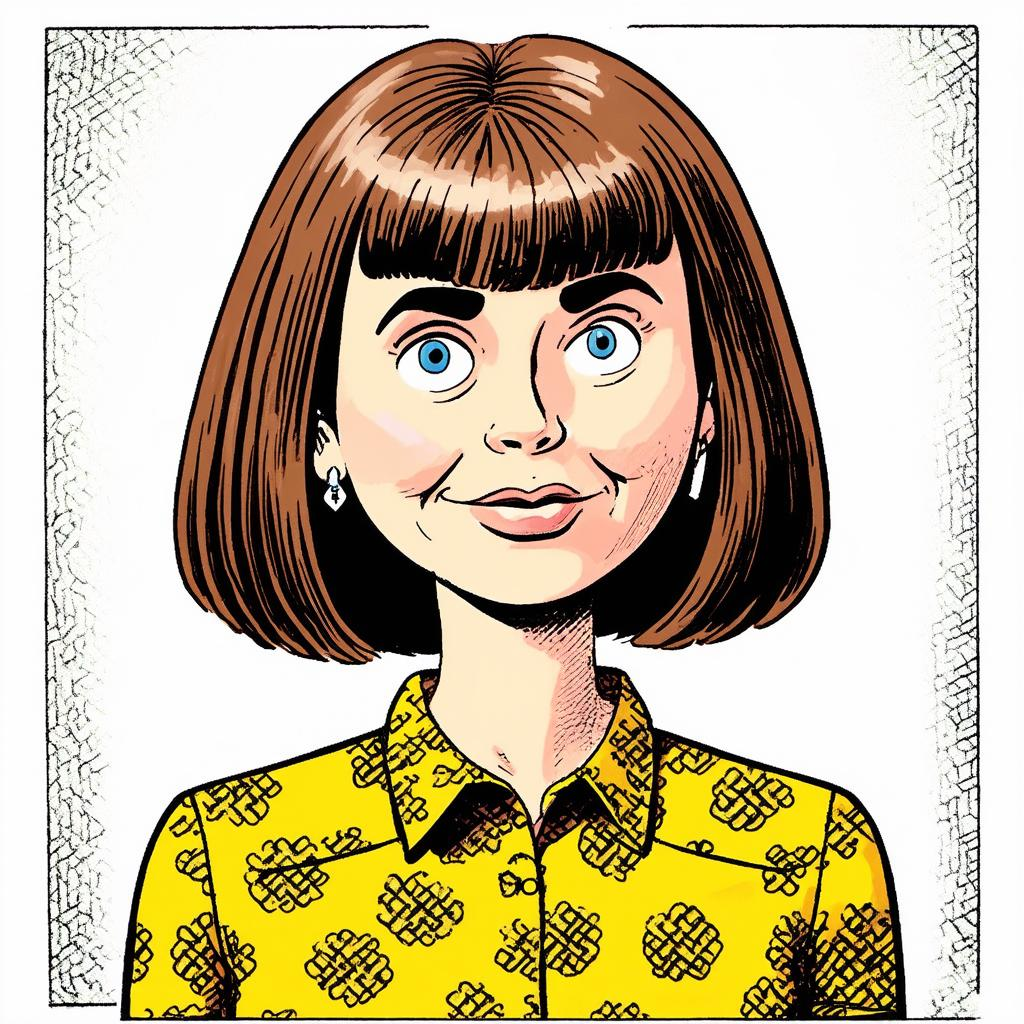
\includegraphics[height=1.9cm]{000009_diff3}
						\end{subfigure}
						\hfill
						\begin{subfigure}[b]{0.18\textwidth}
							\centering
							
\includegraphics[height=1.9cm]{000077_diff3}
						\end{subfigure}
						\hfill
						\begin{subfigure}[b]{0.18\textwidth}
							\centering
							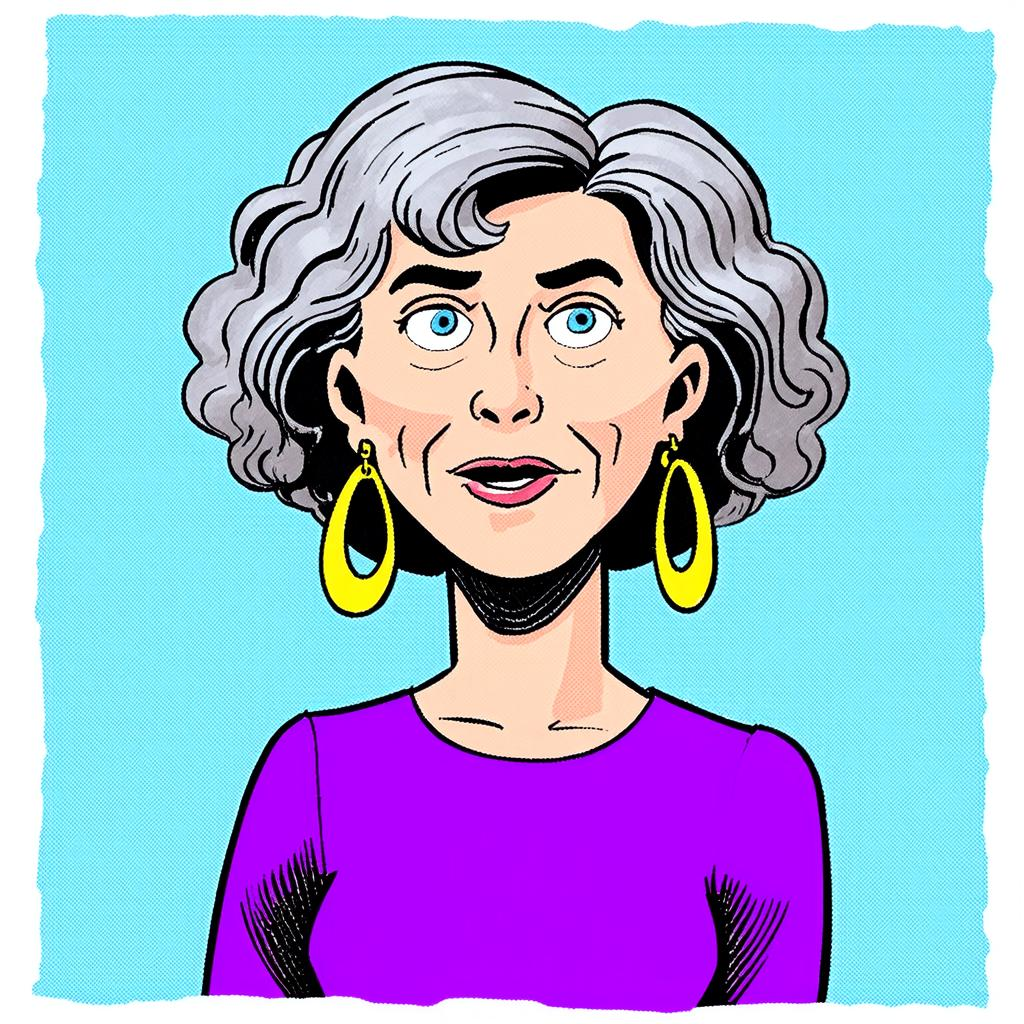
\includegraphics[height=1.9cm]{000084_diff3}
						\end{subfigure}

					\end{minipage}
					\caption{Task 2-1: Failure samples}
				\end{figure}
			\item I tried to generate detailed captions so that the text-to-image (T2I) model would receive as many instructions as possible. I achieved this by asking the model not to describe the background but to focus on the avatar. This did not lead to a significant improvement. Then I tried to improve performance by clarifying the prompt to indicate a ``Peanuts comic'' style (I was worried the model might interpret ``peanut'' as ``groundnut''). It did not work better either. In conclusion, I think zero-shot usage of Stable Diffusion might not yield a significant improvement.
		\end{enumerate}
\end{enumerate}
\newpage
\section*{Task 2-2}
\begin{enumerate}
	\item Briefly describe how you implement task 2-2:
		\begin{itemize}
			\item Generated the captions by Phi-4 beforehand and stored in a json file.
			\item Padded or resized image to 512 $\times$ 512.
			\item Used \textcolor{blue}{\texttt{diffusers.StableDiffusionImg2ImgPipeline}}.
		\end{itemize}
	\item Visualization:
		\begin{enumerate}
			\item You can see an example in Figure 1-c.
			\item Below are examples of success and failure. In the success samples, the face orientation, clothes, and hair color are correctly displayed—although the fourth sample generated the wrong gender, it still captured many relevant features. In the failure samples, most of them fail to generate a proper face.
				\begin{figure}[h!]
					\centering
					\begin{minipage}{0.8\textwidth}
						\centering

						% Row 1
						\begin{subfigure}[b]{0.18\textwidth}
							\centering
							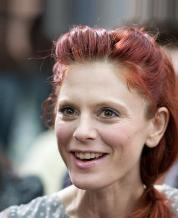
\includegraphics[height=1.9cm]{000002}
						\end{subfigure}
						\hfill
						\begin{subfigure}[b]{0.18\textwidth}
							\centering
							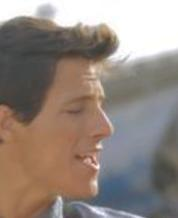
\includegraphics[height=1.9cm]{000003}
						\end{subfigure}
						\hfill
						\begin{subfigure}[b]{0.18\textwidth}
							\centering
							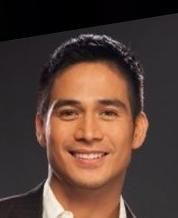
\includegraphics[height=1.9cm]{000012}
						\end{subfigure}
						\hfill
						\begin{subfigure}[b]{0.18\textwidth}
							\centering
							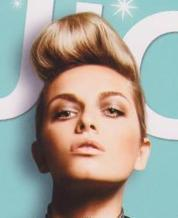
\includegraphics[height=1.9cm]{000005}
						\end{subfigure}
						\hfill
						\begin{subfigure}[b]{0.18\textwidth}
							\centering
							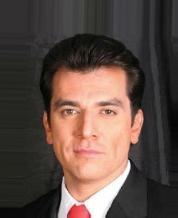
\includegraphics[height=1.9cm]{000055}
						\end{subfigure}

						\vspace{0.6cm} % Space between rows

						% Row 2
						\begin{subfigure}[b]{0.18\textwidth}
							\centering
							
\includegraphics[height=1.9cm]{000002_styled}
						\end{subfigure}
						\hfill
						\begin{subfigure}[b]{0.18\textwidth}
							\centering
							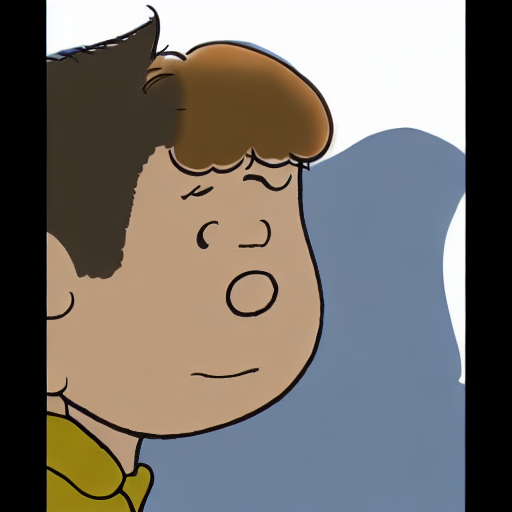
\includegraphics[height=1.9cm]{000003_styled}
						\end{subfigure}
						\hfill
						\begin{subfigure}[b]{0.18\textwidth}
							\centering
							
\includegraphics[height=1.9cm]{000012_styled}
						\end{subfigure}
						\hfill
						\begin{subfigure}[b]{0.18\textwidth}
							\centering
							
\includegraphics[height=1.9cm]{000005_styled}
						\end{subfigure}
						\hfill
						\begin{subfigure}[b]{0.18\textwidth}
							\centering
							
\includegraphics[height=1.9cm]{000055_styled}
						\end{subfigure}

						\caption{Task 2-1: Success samples}
						\vspace{0.6cm} % Space between rows

						% Row 1
						\begin{subfigure}[b]{0.18\textwidth}
							\centering
							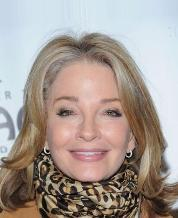
\includegraphics[height=1.9cm]{000018}
						\end{subfigure}
						\hfill
						\begin{subfigure}[b]{0.18\textwidth}
							\centering
							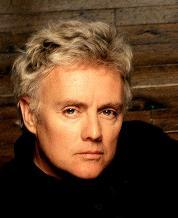
\includegraphics[height=1.9cm]{000030}
						\end{subfigure}
						\hfill
						\begin{subfigure}[b]{0.18\textwidth}
							\centering
							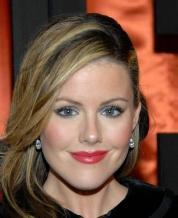
\includegraphics[height=1.9cm]{000042}
						\end{subfigure}
						\hfill
						\begin{subfigure}[b]{0.18\textwidth}
							\centering
							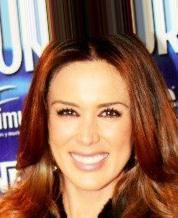
\includegraphics[height=1.9cm]{000045}
						\end{subfigure}
						\hfill
						\begin{subfigure}[b]{0.18\textwidth}
							\centering
							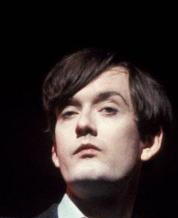
\includegraphics[height=1.9cm]{000048}
						\end{subfigure}

						\vspace{0.6cm} % Space between rows

						% Row 2
						\begin{subfigure}[b]{0.18\textwidth}
							\centering
							
\includegraphics[height=1.9cm]{000018_styled}
						\end{subfigure}
						\hfill
						\begin{subfigure}[b]{0.18\textwidth}
							\centering
							
\includegraphics[height=1.9cm]{000030_styled}
						\end{subfigure}
						\hfill
						\begin{subfigure}[b]{0.18\textwidth}
							\centering
							
\includegraphics[height=1.9cm]{000042_styled}
						\end{subfigure}
						\hfill
						\begin{subfigure}[b]{0.18\textwidth}
							\centering
							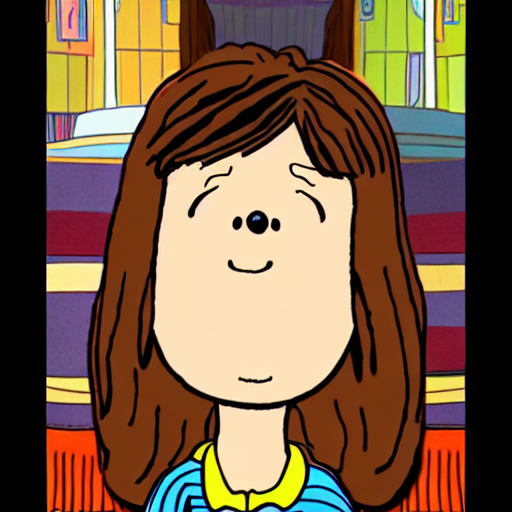
\includegraphics[height=1.9cm]{000045_styled}
						\end{subfigure}
						\hfill
						\begin{subfigure}[b]{0.18\textwidth}
							\centering
							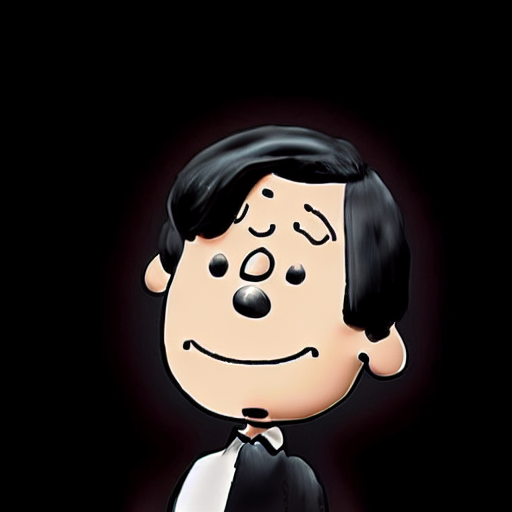
\includegraphics[height=1.9cm]{000048_styled}
						\end{subfigure}

					\end{minipage}
					\caption{Task 2-1: Failure samples}
				\end{figure}
			\item In \textcolor{blue}{\texttt{diffusers.StableDiffusionImg2ImgPipeline}}, there are two tunable parameters: \textcolor{blue}{\texttt{strength}} and \textcolor{blue}{\texttt{guidance\_scale}}. I experimented with several combinations. With lower \texttt{strength} and \texttt{guidance\_scale}, the generated image retains more features from the original content image but shows less of the Peanuts style. This trade-off is something we must consider.
		\end{enumerate}
\end{enumerate}

\end{document}

